\documentclass{article}
\usepackage[utf8]{inputenc}
\usepackage{datetime}
\usepackage{enumerate}
\usepackage{textcomp}
\usepackage{amsmath}
\usepackage{tikz}
\usetikzlibrary{arrows}
\usepackage{graphicx}
\usepackage{amssymb}
\graphicspath{ {./images/} }
   
\title{\bf \Large ASSIGNMENT 7}
\author{Xinhao Luo}
\date{\today}

\def\math#1{$#1$} 

\setlength{\textheight}{8.5in}
\setlength{\textwidth}{6.5in}
\setlength{\oddsidemargin}{0in}
\setlength{\evensidemargin}{0in}
\voffset0.0in

\begin{document}
\maketitle
\medskip

\section{Question 1}

The classification algorithm: Linear Regression for classification followed by pocket for improvement.

Math definition from previous homework:
\begin{itemize}
    \item [up-down symmetry] \math{\sum_{i = 0}^{15}\sum_{j = 0}^{15}|pixel[i][j] - pixel[15 - i][j]|} 
    \item [intensity] \math{\sum_{i = 0}^{15}\sum_{j = 0}^{15}pixel[i][j]}
\end{itemize}

\begin{enumerate}[a)]
    \item 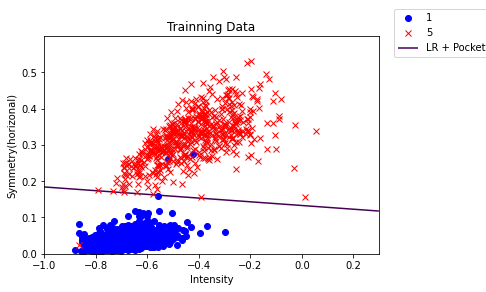
\includegraphics[]{1/1} 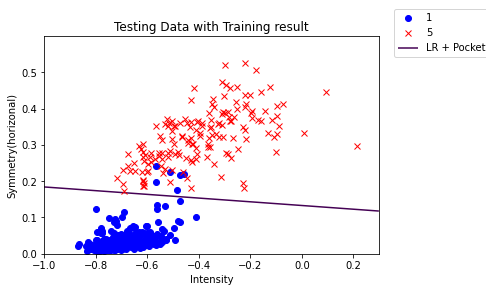
\includegraphics[]{1/2}
    \item 
        \begin{itemize}
            \item [\math{E_{in}}] 0.0019218449711723151
            \item [\math{E_{test}}] 0.014150943396226467
        \end{itemize}
    \item We have 2 features, so \math{d_{vc} = 2 + 1 = 3}. The total number of training set is 1561, and the number of test set is 424. \math{\delta = 0.05}
        \begin{itemize}
            \item [Train] 
                \begin{equation}
                    \begin{split}
                        E_{out} &\leq E_{in} + \sqrt{\frac{8}{N}ln\frac{4((2N)^{d_{vc}} + 1)}{\delta}} \\
                        &\leq 0.00192 + \sqrt{\frac{8}{1561}ln\frac{4((2 * 1561)^3 + 1)}{0.05}} \\
                        &\leq 0.3842
                    \end{split}
                \end{equation}
            \item [Test] \begin{equation}
                    \begin{split}
                        E_{out} &\leq E_{test} + \sqrt{\frac{1}{2N}ln\frac{2M}{\delta}} \\
                        &\leq 0.01415 + \sqrt{\frac{1}{2 * 424}ln\frac{1 * 2}{0.05}} \\
                        &\leq 0.0801
                    \end{split}
                \end{equation}
            Bound based on \math{E_{test}} is better
        \end{itemize}
    \item The 3rd transformation will be \math{(x_0, x_1, x_2, x_1^2, x_2^2, x_1x_2, x_1^3, x_2^3, x_1x_2^2, x_1^2x_2)}
        \begin{enumerate}[a)]
            \item 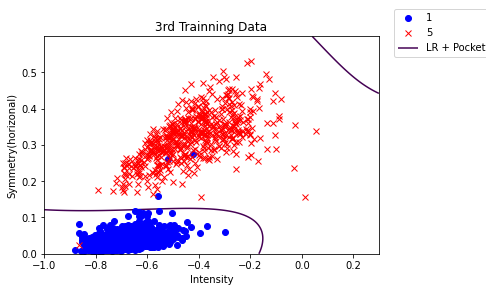
\includegraphics[]{1/3} 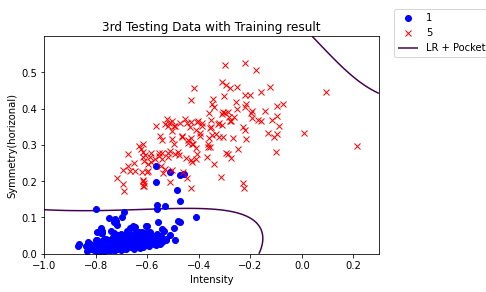
\includegraphics[]{1/4}
        \item 
            \begin{itemize}
                \item [\math{E_{in}}] 0.002562459961563124
                \item [\math{E_{test}}] 0.014150943396226467
            \end{itemize}
        \item We have 2 features, so \math{d_{vc} = 2 + 1 = 3}. The total number of training set is 1561, and the number of test set is 424. \math{\delta = 0.05}
            \begin{itemize}
                \item [Train] 
                    \begin{equation}
                        \begin{split}
                            E_{out} &\leq E_{in} + \sqrt{\frac{8}{N}ln\frac{4((2N)^{d_{vc}} + 1)}{\delta}} \\
                            &\leq 0.00256 + \sqrt{\frac{8}{1561}ln\frac{4((2 * 1561)^3 + 1)}{0.05}} \\
                            &\leq 0.3849
                        \end{split}
                    \end{equation}
                \item [Test] \begin{equation}
                        \begin{split}
                            E_{out} &\leq E_{test} + \sqrt{\frac{1}{2N}ln\frac{2M}{\delta}} \\
                            &\leq 0.01415 + \sqrt{\frac{1}{2 * 424}ln\frac{1 * 2}{0.05}} \\
                            &\leq 0.0801
                        \end{split}
                    \end{equation}
                Bound based on \math{E_{test}} is better
            \end{itemize}
        \end{enumerate}
    \item I would choose to the linear model as the data is separated pretty well already and not necessary to raise to 3rd (didn't gain much improvement). Also, linear model has better error bar and avoid fitting noise. With the number of data we have, choosing a simpler model is more preferred.
\end{enumerate}

\section{Question 2}

\begin{enumerate}
    \item From \math{f(x, y) = x^2 + 2y^2 + 2sin(2\pi x)sin(2\pi y)}, we may have:
    \begin{equation}
        \frac{df(x)}{dx} = 2x + 4\pi cos(2\pi x)sin(2\pi y)
    \end{equation}
    \begin{equation}
        \frac{df(y)}{dy} = 2y + 4\pi sin(2\pi x)cos(2\pi y)
    \end{equation}
    then we may have 
    \begin{equation}
        x_{t + 1} = x_t - \eta (2x_t + 4\pi cos(2\pi x_t)sin(2\pi y_t))
    \end{equation}
    \begin{equation}
        y_{t + 1} = y_t - \eta (2y_t + 4\pi sin(2\pi x_t)cos(2\pi y_t))
    \end{equation} \\
    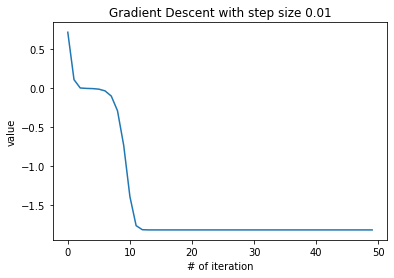
\includegraphics[]{2/1} \\ 
    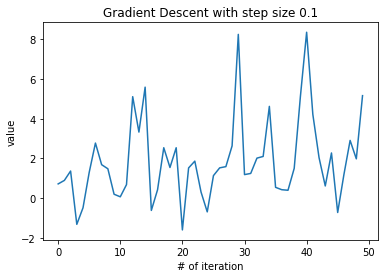
\includegraphics[]{2/2} \\
    For \math{\eta = 0.1}, the value is bouncing around and unable to find the minimum.
    \item The table is listed as below:
        \begin{verbatim}
Initial Point  eta            x              y              Minimum Value  
(0.1, 0.1)     0.1            0.2065         -0.1715        -1.5949        
(0.1, 0.1)     0.01           0.2438         -0.2379        -1.8201        
(1, 1)         0.1            0.1974         -0.2668        -1.6998        
(1, 1)         0.01           1.2181         0.7128         0.5933         
(-0.5, -0.5)   0.1            0.2863         -0.3315        -1.3965        
(-0.5, -0.5)   0.01           -0.7314        -0.2379        -1.3325        
(-1, -1)       0.1            -0.1974        0.2668         -1.6998        
(-1, -1)       0.01           -1.2181        -0.7128        0.5933              
\end{verbatim}
        With different initial points, the minimum value varies, so it is hard to locate the "true" global minimum of an arbitrary function.
\end{enumerate}

\section{Problem 3.16}

\begin{enumerate}
    \item Since \math{g(x) = P[y = +1|x]}, then \math{P[y = -1|x] = 1 - g(x)}
        \begin{equation}
            \begin{split}
                cost(accept) &= P[y = -1|x] * C_a + P[y = +1|x] * 0 \\
                &= (1 - g(x))C_a
            \end{split}
        \end{equation}
        \begin{equation}
            \begin{split}
                cost(reject) &= P[y = -1|x] * 0 + P[y = +1|x] * C_r \\
                &= g(x)C_r
            \end{split}
        \end{equation}
    \item If \math{cost(reject) \geq cost(accept)}, we accept the person. Thus we may have:
    \begin{equation}
        \begin{split}
            g(x)C_r &\geq (1 - g(x))C_a \\
            g(x)C_r &\geq C_a - g(x)C_a \\
            g(x)C_r + g(x)C_a &\geq C_a \\
            g(x)(C_r + C_a) &\geq C_a \\
            g(x) &\geq \frac{C_a}{(C_r + C_a)}
        \end{split}
    \end{equation}
    Thus, \math{k = \frac{C_a}{(C_r + C_a)}}
    \item Data from Example 1.1
        \begin{itemize}
            \item [Supermarket] \math{C_a = 1} and \math{C_r = 10}, thus
            \begin{equation}
                k = \frac{1}{10 + 1} \approx 0.0909
            \end{equation}
            \item [CIA] \math{C_a = 1000} and \math{C_r = 1}, thus
            \begin{equation}
                k = \frac{1000}{1000 + 1} \approx 0.9990
            \end{equation}
        \end{itemize}
        The high threshold means low toleration to false positive. Thus for CIA, intruders will cause way more troubles than some people falsely rejected. While the supermarket could accept giving discount to non-target customer, but if falsely rejected a customer, the supermarket will possibly lose the customer forever, thus a low threshold is set.
\end{enumerate}

\end{document}
